\subsection{Martian application}
With regard to the usability of the modeled energy distribution for a self-sufficient voice communication system on the surface of Mars, roughly speaking, two main components have to be examined more closely. Namely the PV generator and the $\mathrm{LiFePO}_4$ battery.

Since Mars, with an average distance of $1,524\mathrm{AU}$, is further away from the Sun than the Earth, the solar irradiance $E_\mathrm{S,M}$ in $\left(\mathrm{Wm^{-2}}\right)$ at the top of its atmosphere is $56,9\%$ less than that on Earth \cite{Karttunen:2006}: 
\begin{equation} \label{eq:e_sun_mars}
	\centering
	E_{\mathrm{S,M}} = \frac{\Phi_{\mathrm{S}}}{4 \pi \, \left(1,524 \cdot r_{\mathrm{SE}}\right)^2} = \frac{3,845 \cdot 10^{26} \mathrm{W}}{4 \pi \cdot (2,279871539 \cdot 10^{11} \mathrm{m})^2} = 588,66 \frac{\mathrm{W}}{\mathrm{m}^2}\text{.}
\end{equation}
Similar to the solar resource maps introduced in the subsection \ref{sec:solar_irradiation_on_earths_surface}, the Solar irradiance data collected by NASA's Viking Lander VL1, shown in the figures \ref{fig:image_mars_irradiance_mean} to \ref{fig:image_mars_irradiance_orbit}, can be used to calculate the total generator irradiance on the Martian surface, based on the equations (\ref{eq:e_dni}) and (\ref{eq:e_gen_ghi_dni}):
\begin{equation} \label{eq:e_gen_ghi_dni_mars}
	\centering
		E_{\mathrm{G}}(t_\mathrm{S}) = E_{\mathrm{DHI}} \, \dfrac{\cos \theta}{\sin \gamma_\mathrm{S}} + E_{\mathrm{DIFH}} \,\frac{1 + \cos \beta }{2} + E_{\mathrm{GHI}} \, \frac{1 - \cos \beta }{2} \cdot \mathrm{ALB} \text{.}
\end{equation}
\begin{figure}[h!]
	\centering
  	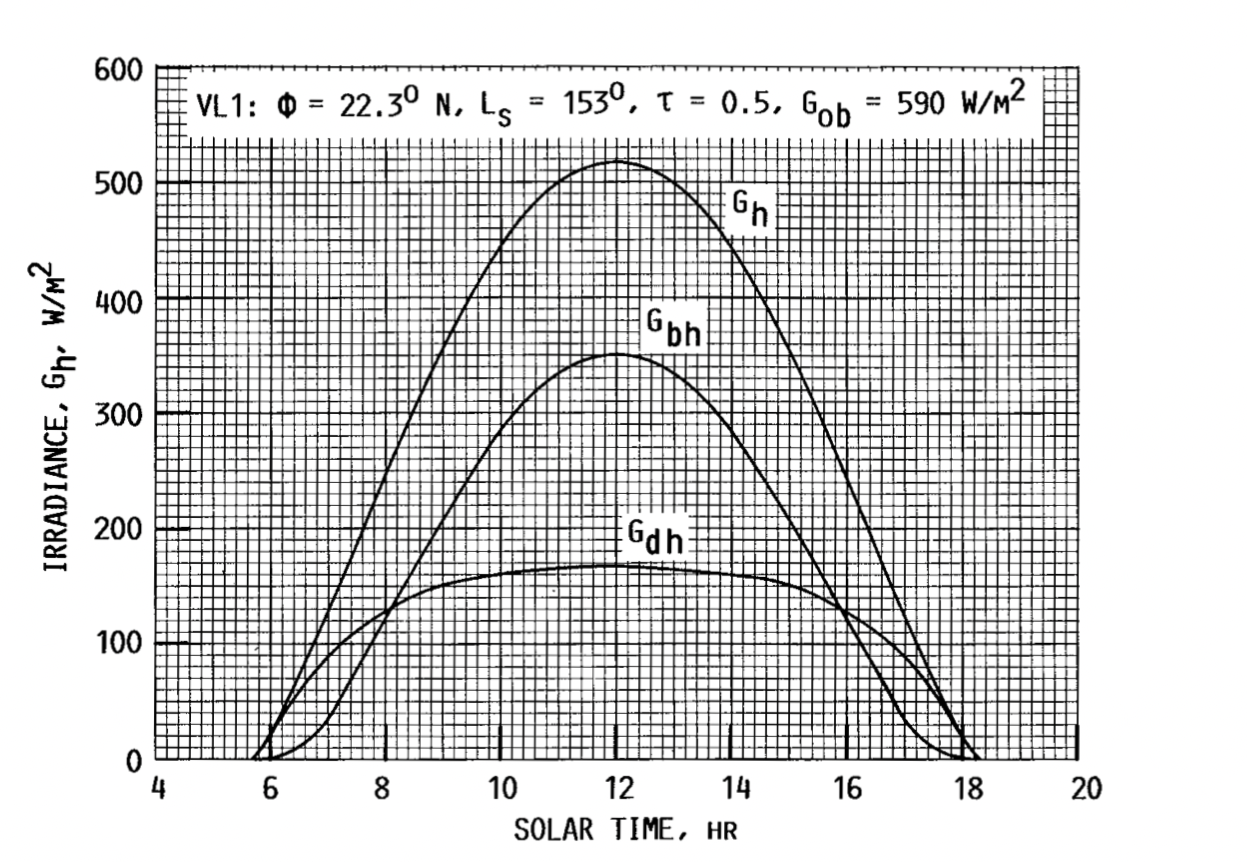
\includegraphics[width = 0.9\textwidth]{images/image_mars_irradiance_mean}
  	\caption{\textit{``Diurnal variation of global $G_\mathrm{h}$, beam $G_\mathrm{bh}$ and diffuse $G_\mathrm{dh}$ irradiance on a horizontal Mars surface at Viking Lander VL1.''} (Image and caption credit: \cite{Appelbaum:1990})}
	\label{fig:image_mars_irradiance_mean}
\end{figure}
The quantities $E_{\mathrm{DHI}}$, $E_{\mathrm{DIFH}}$, $E_{\mathrm{GHI}}$, $\theta$ and $\gamma_\mathrm{S}$ depend on the solar time $t_\mathrm{S}$. As a first approximation, the albedo value $\mathrm{ALB} = 0,25$ can be used. This value represents the mean albedo of Mars \cite{Grayzeck:2020}. In the article \cite{Appelbaum:1990} the authors further state that the albedo of the Martian surface varies in the range of $0,1$ to $0,4$.

The data presented in the figures \ref{fig:image_mars_irradiance_mean} to \ref{fig:image_mars_irradiance_orbit}, however, only applies for the Martian latitude $\phi \ \widehat{=} \ \varphi = 22,3^\circ \, \mathrm{N}$. Figure \ref{fig:image_mars_irradiance_mean} shows the diurnal variation of $E_{\mathrm{DHI}} \ \widehat{=} \ G_\mathrm{bh}$, $E_{\mathrm{DIFH}} \ \widehat{=} \ G_\mathrm{dh}$ and $E_{\mathrm{GHI}} \ \widehat{=} \ G_\mathrm{h}$ on the Martian surface. The quantities $L_\mathrm{S}$, $\tau$ and $G_\mathrm{ob}$ are the areocentric longitude, the optical depth and the beam irradiance at the top of the Martian atmosphere. Similar data is shown in the figures \ref{fig:image_mars_irradiance_orbit} and \ref{fig:image_mars_irradiance_opacity}, but here an additional reference is made to the orbit of Mars around the Sun and the opacity of its atmosphere. For example, the latter can be caused by dust storms \cite{Appelbaum:1990}. 
\begin{figure}[h!]
	\centering
  	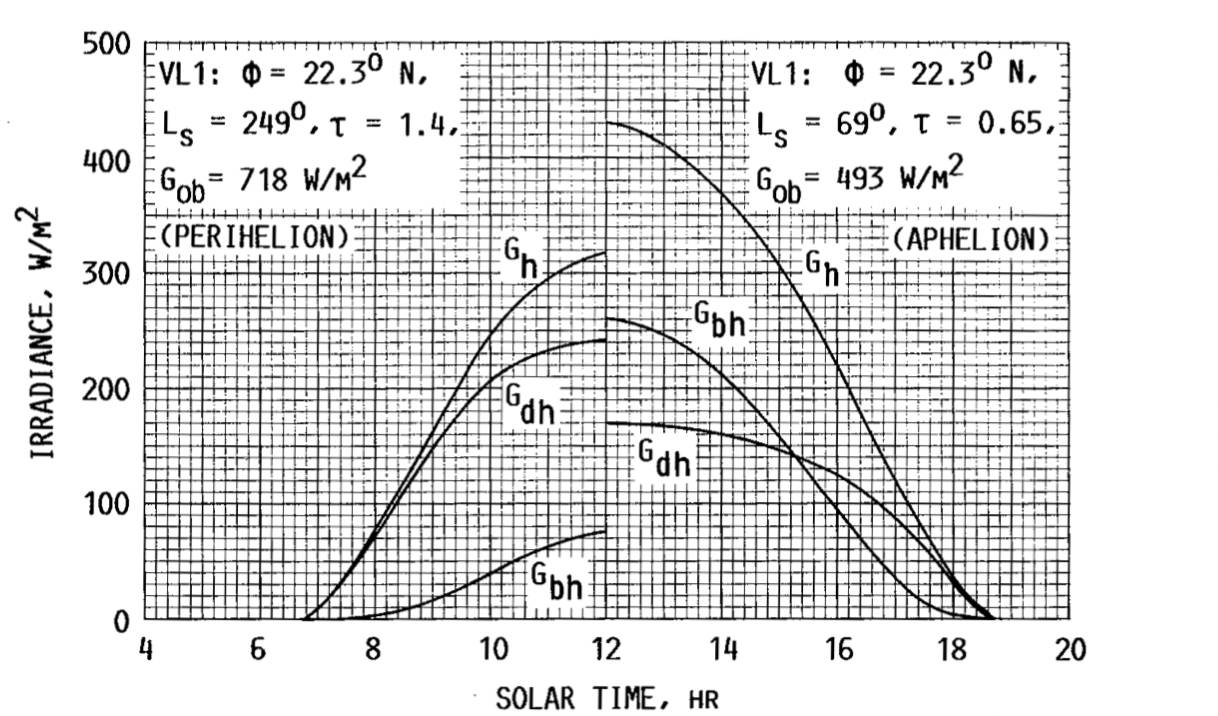
\includegraphics[width = 0.9\textwidth]{images/image_mars_irradiance_orbit}
  	\caption{\textit{``Diurnal variation of global $G_\mathrm{h}$, beam $G_\mathrm{bh}$ and diffuse $G_\mathrm{dh}$ irradiance on a horizontal Mars surface at Viking Lander VL1.''} (Image and caption credit: \cite{Appelbaum:1990})}
	\label{fig:image_mars_irradiance_orbit}
\end{figure}
\begin{figure}[h!]
	\centering
  	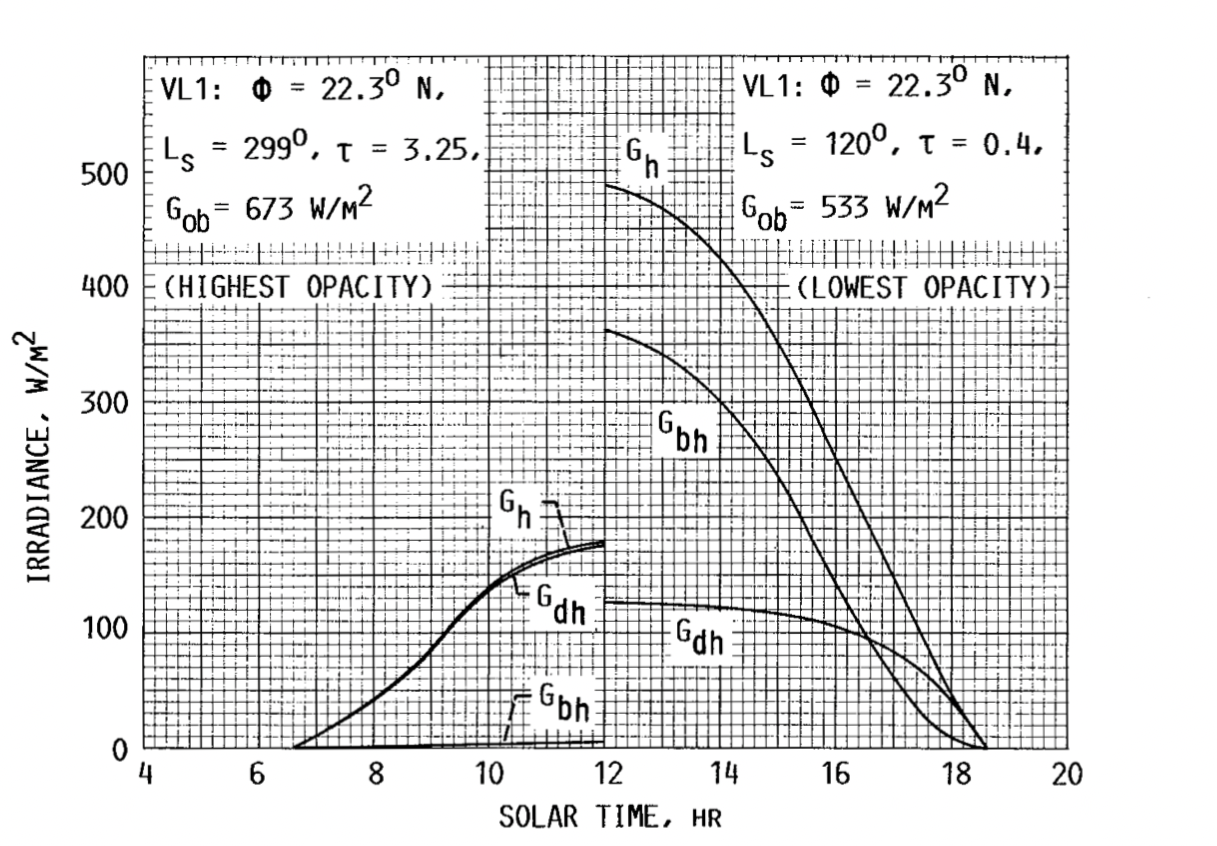
\includegraphics[width = 0.9\textwidth]{images/image_mars_irradiance_opacity}
  	\caption{\textit{``Diurnal variation of global $G_\mathrm{h}$, beam $G_\mathrm{bh}$ and diffuse $G_\mathrm{dh}$ irradiance on a horizontal Mars surface at Viking Lander VL1.''} (Image and caption credit: \cite{Appelbaum:1990})}
	\label{fig:image_mars_irradiance_opacity}
\end{figure}

The angles $\theta$ and $\gamma_\mathrm{S}$ can be calculated with the equations introduced in the subsections \ref{sec:angular_relationships} and \ref{sec:energy_yield}. For these, however, the local latitude $\varphi$, the Sun's declination $\delta$ and the solar time $t_\mathrm{S}$ on Mars must be known. On Mars, the maximum values of $\delta$ are $-25,19^\circ$ and $25,19^\circ$ and the duration of one day is $24,6597\mathrm{h}$ \cite{Grayzeck:2020}. It is noted, that the equations (\ref{eq:delta}) and (\ref{eq:solar_time}) cannot be used to calculate $\delta$ and $t_\mathrm{S}$.

In order to get the same energy yield with a PV generator on Mars as on Earth, this can be achieved in two ways. Based on the equation (\ref{eq:radiation_flux}), and if it is assumed that the PV cell temperatures of the PV generator on Earth and Mars are equal ($\vartheta_\mathrm{C,E} = \vartheta_\mathrm{C,M}$), the radiation flux onto the energy-converting area $A_\mathrm{PV,E}$ of the PV generator on Earth is equal to the radiation flux onto the energy-converting area $A_\mathrm{PV,M}$ of the PV generator on Mars, when the following equation applies:
\begin{equation} \label{eq:pv_area_comparison}
	\centering
		A_{\mathrm{PV,M}} = A_{\mathrm{PV,E}} \, \dfrac{E_{\mathrm{G,E}}}{E_{\mathrm{G,M}}}\text{,} \quad \text{for } \vartheta_\mathrm{C,E} = \vartheta_\mathrm{C,M} \text{.}
\end{equation}
Therefore, a self-sufficient voice communication system with a PV generator area $A_{\mathrm{PV,E}}$ and, for example, the requirement of an annual average irradiance $E_{\mathrm{G,E}}$ to operate on Earth, would require an area $A_{\mathrm{PV,M}}$ if there is an annual avarege irradiance $E_{\mathrm{G,M}}$ at the place of use on Mars. The main disadvantage of this method is, that as the area of the PV generator increases, its mass and thus the payload of a rocket increases. 

Diurnal temperatures between $-89^\circ \mathrm{C}$ to $-31^\circ \mathrm{C}$ on Mars theoretically lead to a higher output power of the PV generator. This can reduce the required area $A_{\mathrm{PV,E}}$ \cite{Mertens:2015, Grayzeck:2020}. However, the influence of temperature must be examined more closely. Altough the ambient temperature is lower, the heat dissipation of the PV generator to the surrounding atmosphere is worse than on Earth \cite{Kemmetmuller:2021}. This shows that the equation (\ref{eq:pv_area_comparison}) can only be used as a rough estimate.

The second approach is based on increasing the sensitivity $S$ of the PV cells (see equation (\ref{eq:sens})) so that equation the (\ref{eq:photo_i}) can still deliver the same photocurrent current to charge the $\mathrm{LiFePO}_4$ battery at a lower radiation flux $\Phi_\mathrm{G}$. In order to achieve this, the structure of the semiconductor the PV cells are made of needs to be adapted and improved. Research is still ongoing in this area \cite{Mertens:2015}.  

With regard to longer lasting dust storms, energy can still be converted to supply the self-sufficient voice communication system due to the diffuse component of the total generator irradiance (compare to figure \ref{fig:image_mars_irradiance_opacity}). This must be planned accordingly \cite{Appelbaum:1990, Appelbaum:1992, Landis:1995, Mertens:2015}. It becomes more complicated when dust collects on the energy-converting area of the PV generator. Crew members would have to dust it off from time to time. This, however, shortens the effective mission time and increases the risk of an accident. Regarding the $\mathrm{LiFePO}_4$ battery, this can further become a problem in between crewed missions. Even though these types of batteries have a low self-discharge, they can get damaged if they are not sufficiently charged for a longer period of time \cite{Offgridtec:2020}.

Finally, the second component that is heavily influenced by the Martian environment is the $\mathrm{LiFePO}_4$ battery. This is mainly due to the aforementioned extreme diurnal ambient temperatures \cite{Hausmann:2013, Wehbe:2015, Ala-A.-Hussein:2015, Nejad:2016, Chin:2018, Grayzeck:2020}. Depending on how well the battery is insulated from the Martian environment in terms of temperature, additional energy from the battery must be used to continuously heat or cool it. Due to this, the nominal battery charge and -- if necessary -- the energy-converting area of the PV generator must be adjusted. 
